\section{Introduction}

Recommendation systems are a vital component of the modern Web.  They
help readers effectively navigate otherwise unwieldy archives of
information and help websites direct users to items---movies,
articles, songs, products---that they will like.
A recommendation system is built from user behavior data, historical
data about which items each user has consumed, be it clicked, viewed,
rated, or purchased. First, we uncover the behavioral patterns that
characterize various types of users and the kinds of items they tend
to like.  Then, we exploit these discovered patterns to recommend
future items to its users.

In this paper, we develop Poisson factorization (PF) algorithms for
recommendation.  Our algorithms easily scale to massive data and
significantly outperform the existing state of the art.  We show that
Poisson factorization for recommendation is tailored to real-world
properties of user behavior data: the heterogenous interests of users,
the varied types of items, and a realistic distribution of the finite
resources that users have to consume items.

Figure 1 illustrates Poisson factorization on data from Netflix.  The
Netflix data contains the ratings of 480,000 users on 17,000 movies,
organized in a matrix of 8.16B cells (and containing 250M ratings).
From these data, we extract the patterns of users' interests and the
movies that are associated with those interests.  The left panel
ilustrates some of those patterns---the algorithm has uncovered genres
of comedies, classic movies, and 1980s stoner movies.

The right panel illustrates how we can use these patterns to form
recommendations for an (imaginary) user.  This user enjoys various
types of movies, including war movies (like ``Breaker Morant'') and
romantic dramas (like ``Leaving Las Vegas'').  Of course, she has only
seen a handful of the available movies.  PF first uses the movies she
has seen to infer what kinds of movies she is interested in, and then
uses these inferred interests to suggest movies she has not yet seen.
The list of movies at the bottom of the figure was suggested by our
algorithm. It includes other war dramas (such as ``Apocalypse Now'')
and other romantic movies (such as ``Breakfast at Tiffany's'').

In more detail, Poisson factorization is a probabilistic model of
users and items.  It associates each user with a latent vector of
preferences, each item with a latent vector of attributes, and
constrains both sets of vectors to be sparse and non-negative.  Each
cell of the observed behavior matrix is assumed drawn from a Poisson
distribution---an exponential family distribution over non-negative
integers---whose parameter is a linear combination of the
corresponding user preferences and item attributes.  The main
computational problem is posterior inference: given an observed matrix
of user behavior, we discover the latent attributes that describe the
items and the latent preferences of the users.  For example, the
components in Figure 1 (left) illustrate the top items for specific
attribute dimensions and the plot in Figure 1 (middle) illustrates the
estimated preference vector for the given user.  A spike in the
preference vector means that the user tends to like items with the
corresponding latent attribute.

To readers familiar with recommendation systems, this procedure is
reminiscent of many variants of matrix factorization.  We found,
however, that PF enjoys significant quantitative advantages over
classical methods and for a wide variety of data sets, including those
with implicit feedback (a binary matrix indicating which items users
consumed) and those with explicit feedback (a matrix of integer
ratings).  \myfig{results} shows that PF, and its hierarchical variant
HPF, perform significantly better than state-of-the art
methods---including the industry standard of matrix factorization with
user and item biases (MF)---for large data sets of Netflix users
watching movies, Last.FM users listening to music, scientists reading
papers, and \textit{New York Times} readers clicking on articles.

% dmb: above, add a cite for the industry standard.

There are two main advantages of Poisson factorization over
traditional methods, both of which contribute to its superior
empirical performance.  First, it better captures real consumption
data, specifically that users have finite (and varied) resources with
which to view items.  To see this, we can rewrite the model as a two
stage process where a user first decides on a budget of movies to
watch and then spends this budget watching movies that she is
interested in.  If the model accurately captures the distribution of
budgets then watched items carry more weight than unwatched items,
because unwatched items can be partially explained by a lack of
resources. We conjecture that classical matrix factorization
systematically overestimates the users' budgets, and we confirm this
hypothesis in \mysec{eval} using a posterior predictive
check~\cite{Gelman:1996}.  This misfit leads to an overweighting of
the zeros, which explains why practitioners require complex methods
for downweighting
them~\cite{Hu:2008p9402,Gantner:2012p9364,Dror:2012a,Paquet:2013p9197}.
(We used one such method in the study of \myfig{eval}.)  Poisson
factorization does not need to be patched in this way.

The second advantage of PF algorithms is that they need only iterate
over the viewed items in the observed matrix of user behavior, i.e.,
the non-zero elements, and this is true even for implicit or
``positive only'' data sets.  (This follows from the mathematical form
of the Poisson distribution.)  Thus, Poisson factorization takes
advantage of the natural sparsity of user behavior data and can easily
analyze massive real-world data. In contrast, classical matrix
factorization is based on the Gaussian
distribution~\cite{Salakhutdinov:2008} and must iterate over the
entire matrix (especially with implicit data).  Thus it cannot take
advantage of data sparsity, which makes computation difficult for even
modestly sized problems.  For example, one cannot fit to the full
Netflix data set (as we did in Figure 1) without appealing to
stochastic optimization~\cite{Mairal:2010}.  We note that our
algorithms are also amenable to stochastic optimization, which we can
use to analyze data sets even larger than those we studied.

% dmb: add paper organization

We reviewed related work below before discussing details of the
Poisson factorization model, including its statistical properties and
methods for scalable inference on large data sets.

\begin{figure*}[th]
\centering
\caption{The top movies in 3 components of the user $U$ illustrated in
  Fig~\ref{fig:movielens-illustration}.}
\vspace{0.1cm}
\small
\begin{tabular}{c}
\toprule
\bf{``Action''}\\
\midrule
The Matrix\\
The Matrix: Reloaded\\
Spider-Man\\
X2: X-Men United\\
\bottomrule
\end{tabular}
\begin{tabular}{c}
\toprule
\bf{``Comedy, Romance''}\\
\midrule
Grosse Pointe Blank\\
Four Weddings and a Funeral\\
High Fidelity\\
Much Ado About Nothing\\
\bottomrule
\end{tabular}
\begin{tabular}{c}
\toprule
\bf{``Science Fiction''}\\
\midrule
Star Wars: Episode IV: A New Hope\\
Star Wars: Episode VI: Return of the Jedi\\
Star Wars: Episode V: The Empire Strikes Back\\
Back to the Future Part II\\
\bottomrule
\end{tabular}
\end{figure*}

\begin{figure*}
\centering
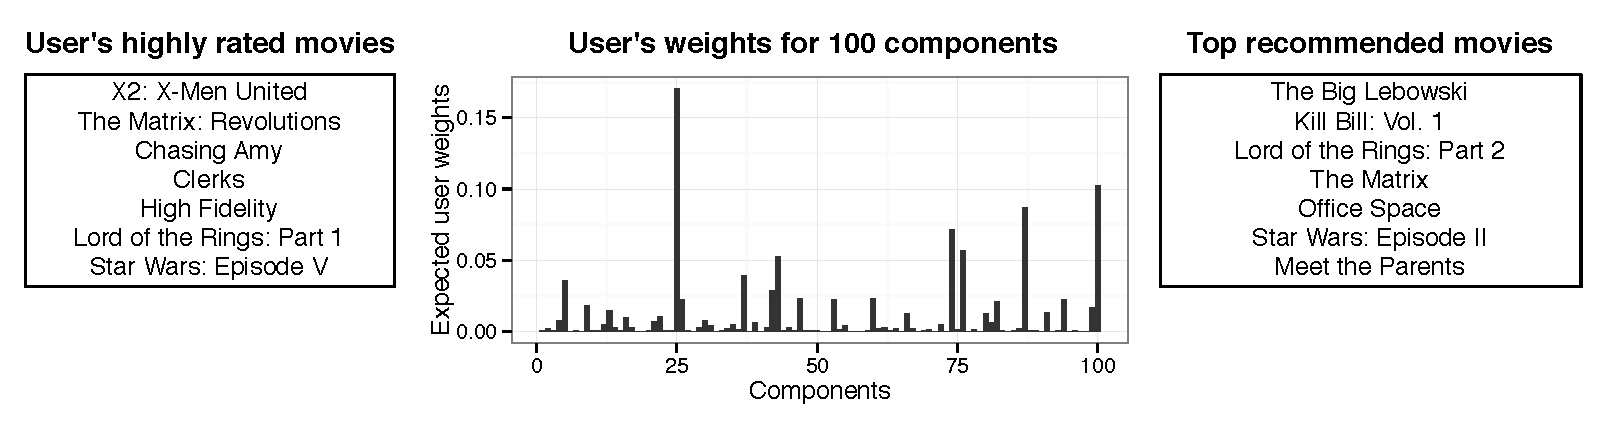
\includegraphics[width=\textwidth]{figures/netflix-exploratory.pdf}\\
\caption{An illustration showing a subset of the highly rated movies
  of a selected user in the Netflix data set~\cite{Koren:2009}, and
  some of the top movies recommended to the user by our algorithm. The
  expected user's $K$-vector of weights $\theta_u$, inferred by our
  algorithm is shown. In our analysis, $K$ was set to 100.}
\label{fig:netflix-illustration}
\end{figure*}


%%
%%\begin{figure}
%%\centering
%%\includegraphics[width=0.8\columnwidth]{figures/movielens-user.pdf}\\
%%\includegraphics[width=0.8\columnwidth]{figures/movielens-item.pdf}\\
%%\caption{The weights of the randomly chosen user $U$ (Top) in the
 %% movielens data set and the weights of her top recommended movie
  %%\emph{Shakespeare in Love} (Bottom) are shown. User $U$ views a
  %%variety of movies, and her weights span a range of factor. User $U$
  %%had 184 views in the data set of movies ranging from Drama, Comedy,
  %%Thriller to Musical. Of these movies, 126 were either 4 or 5
  %%stars. Movies are generally characterized by a sparse set of
  %%factors.}
%%\end{figure}



%% \begin{figure*}[t!]
%% 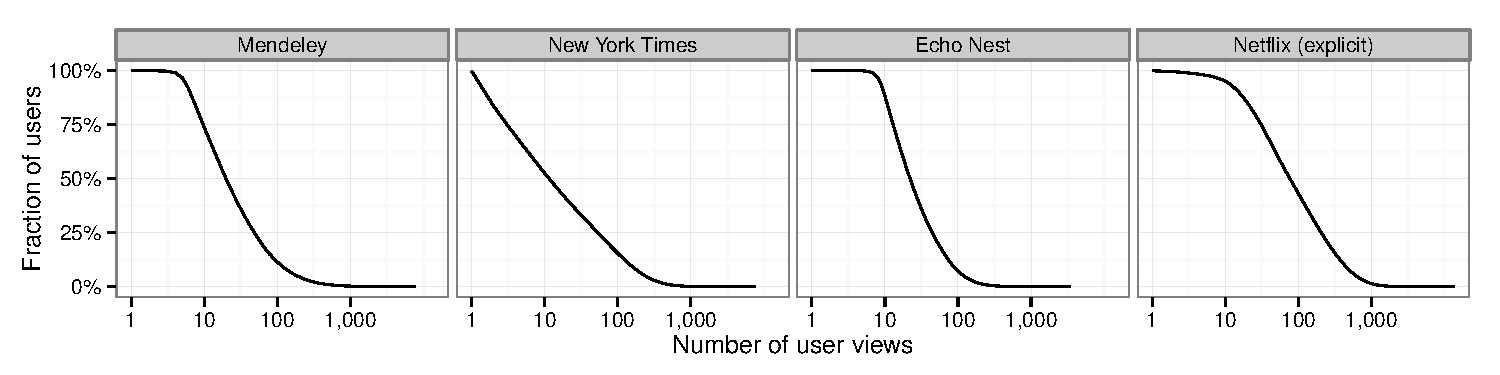
\includegraphics[width=\textwidth]{figures/user_activity_cdf.pdf}
%% \caption{Empirical complimentary cumulative distributions of user
%%   activity on each data set. Each curve shows the fraction of users
%%   who have consumed at least a given number of items. For instance,
%%   slightly less than half of all Netflix users have rated at least
%%   100 movies.}
%% \label{fig:marginals}
%% \end{figure*}


%% \begin{figure*}[t!]
%%   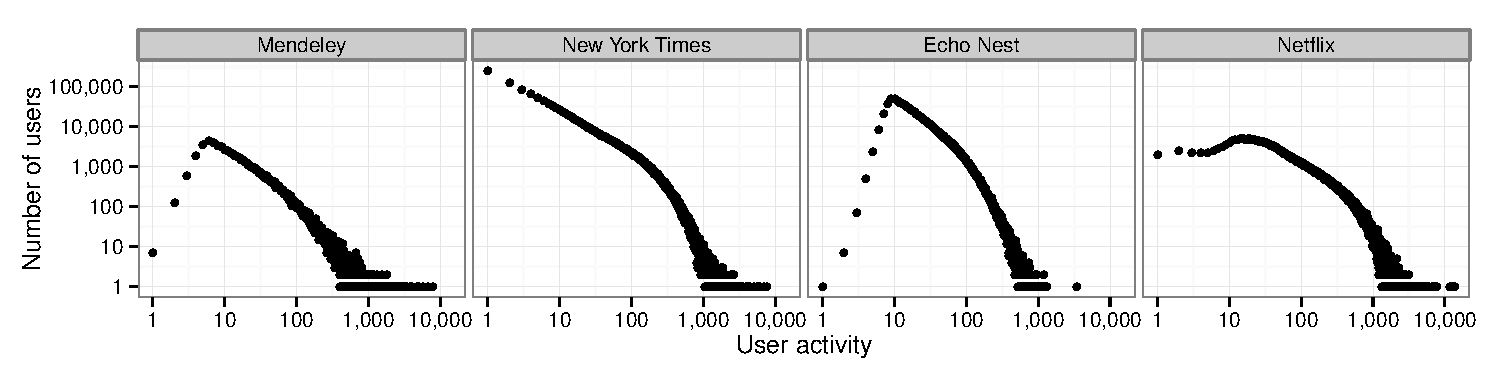
\includegraphics[width=\textwidth]{figures/user_activity.pdf}
%%   \caption{Empirical distributions of user activity on each
%%     dataset. Each plot shows the number of users who have rated a given
%%     number of items. For instance, slightly less than half of all
%%     Netflix users have rated at least 100 movies.}
%% \label{fig:marginals}
%% \end{figure*}


\begin{figure}[t!]
  \centering
  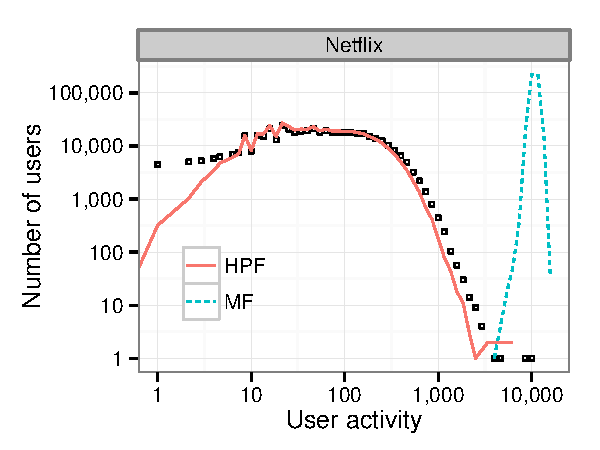
\includegraphics[width=0.4\textwidth]{figures/user_activity_sim_netflix.pdf}
  \caption{The distribution of total ratings for the Netflix dataset.
    The pink curve shows the empirical count of the number of users
    who have rated a given number of items, while the green and blue
    curves show the simulated totals from fitted Poisson and
    traditional matrix factorization models, respectively. The Poisson
    marginal closely matches the empirical, whereas traditional matrix
    factorization fits a large mean to account for skew in the
    distribution.}
\label{fig:marginals}
\end{figure}

%% \begin{figure*}[t!]
%% 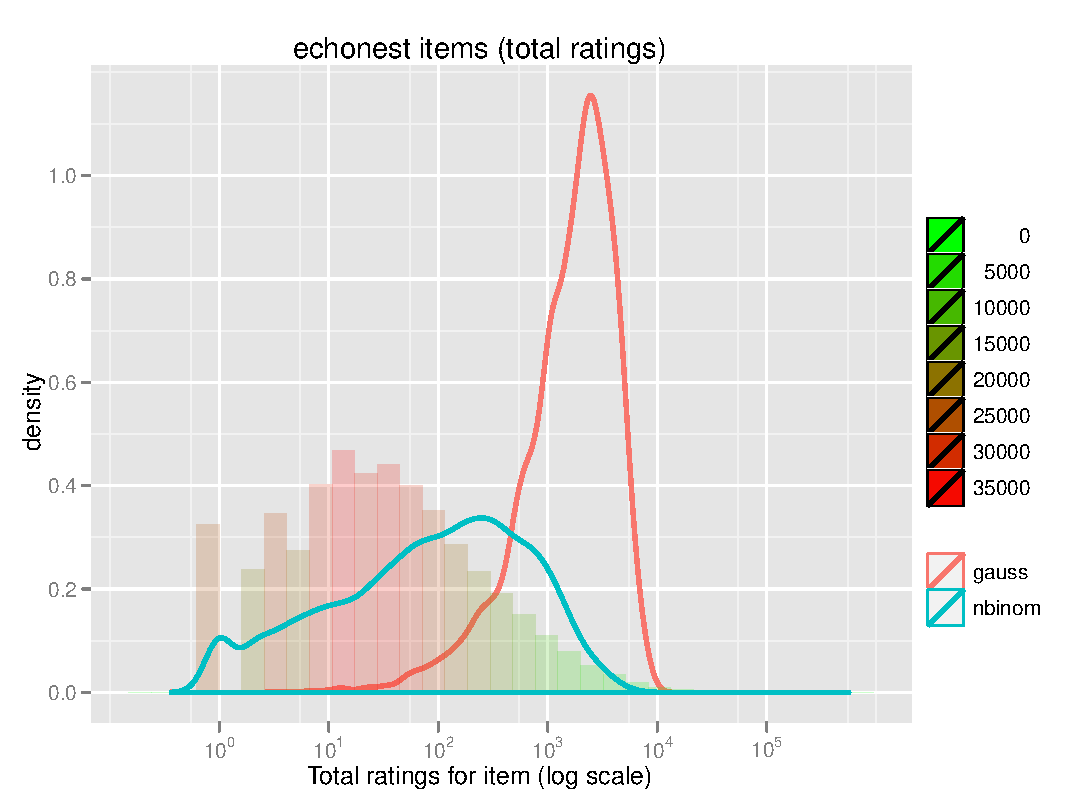
\includegraphics[width=0.33\textwidth]{figures/marginals/echonest.pdf}
%% 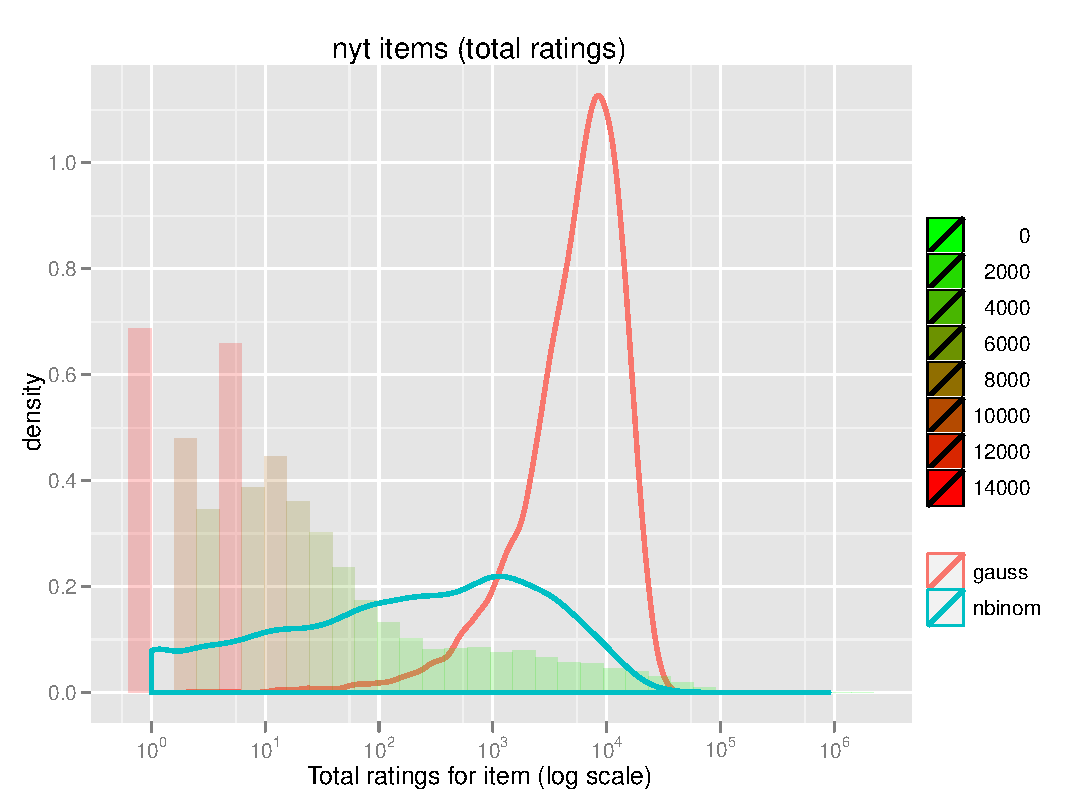
\includegraphics[width=0.33\textwidth]{figures/marginals/nyt.pdf}
%% 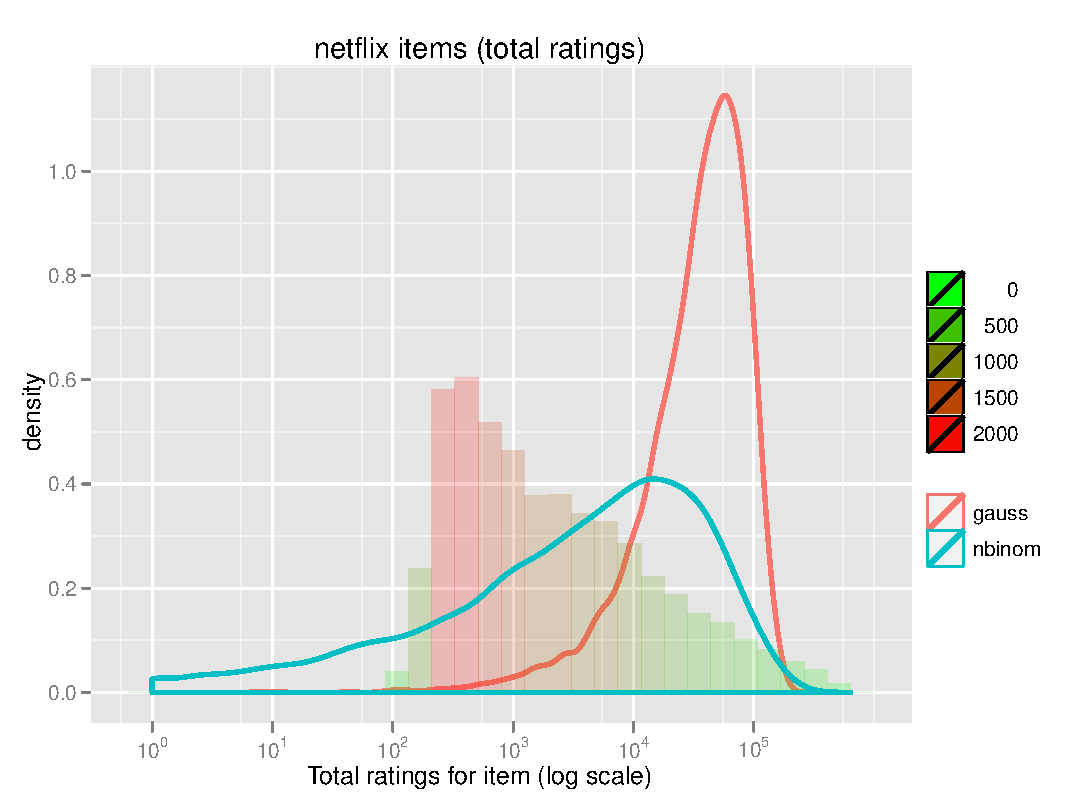
\includegraphics[width=0.33\textwidth]{figures/marginals/netflix.pdf}
%% \caption{Empirical distribution of item popularity on real datasets,
%%   with fitted negative binomial and Gaussian distributions. The
%%   distributions were fit using maximum likelihood estimation. The
%%   negative binomial places significant probability mass on the left
%%   tail, i.e., items with few ratings. The colored bars show that such
%%   items are the most frequent. In contrast, the Gaussian distribution
%%   places negligible mass on the left tail and mainly captures popular
%%   items. The mode of the negative binomial distribution is also closer
%%   to the empirical mode than the Gaussian distribution.}
%% \label{fig:marginals}
%% \end{figure*}

%% Further speed-ups using stochastic variational
%% inference~\cite{Hoffman:2013} let us fit Poisson factorization models
%% to massive data.

